\documentclass[a4paper,11pt]{article}
\usepackage[utf8]{inputenc}
\usepackage[T1]{fontenc}
\usepackage[french]{babel}
\usepackage[right=2.5cm, left=2.5cm, bottom=4cm, top=3cm]{geometry}
\usepackage{textcomp}
\usepackage{graphicx}
\usepackage{mathtools,amssymb,amsthm}
\usepackage{lmodern}
\usepackage{multirow}
\usepackage{array}
\usepackage{longtable}

\title{\vspace{13em}{\huge Cahier des Charges}}
\author{Edouard Fouassier - Maxime Gonthier - Benjamin Guillot\\
		Laureline Martin - Rémi Navarro - Lydia Rodrigez de la Nava
		\vspace{2em}\\
		Algorithme Génétique
		\vspace{2em}}

\begin{document}
	
	\pagenumbering{gobble}\clearpage
	\maketitle\vspace{13em}
\newpage
\tableofcontents
\newpage\clearpage\pagenumbering{arabic}
	
	\section{Introduction}
		Le nom algorithme génétique provient des ressemblances avec le monde du vivant. On utilise des notions telles que la sélection naturelle, les générations ou bien encore la sélection naturelle, dans le but de trouver la meilleure population possible. 
		Cet algorithme a été étudié par John Holland de 1960 à 1975 dans son ouvrage Adaptation in Natural and Artificial System inspiré entre autres par la “learning machine” de Turing.\\
		\\
		L’algorithme génétique s’applique à une grande variété de domaines, tels que la génétique pour étudier l’évolution des gènes d’une espèce donnée sur plusieurs générations. 
		On peut aussi l'appliquer dans le cas d’apprentissage pour par exemple apprendre à un robot à se déplacer en fonction des obstacles, ou bien on peut l'utiliser dans l'optique de trouver un résultat optimisé.
		On peut citer dans cette dernière catégorie l’optimisation d'un portefeuille d'actions en fonction de leur risques, l’optimisation de la ventilation dans le cas d'incendie dans un espace confiné ou bien simplement l’optimisation d’une fonction.\\ 
		\\
		L’algorithme génétique est particulièrement utile lorsque l’utilisateur étudie une population de valeurs et qu’il recherche une solution approchée parmi ces valeurs. 
		Il se démarque des autres algorithmes car il est très facilement adaptable à différents problèmes. 
		De plus, on utilise des règles de transition probabiliste, ce qui est pertinent pour des problèmes où les résultats sont des valeurs approchées.\\

	\section{Fondement du projet}
		\subsection{But du projet}
			L'objectif du projet est de réaliser un programme utilisant un algorithme génétique permettant de délivrer une solution ou un ensemble de solutions optimales à problème donné.
		
		\subsection{Personnes et organismes impliqués dans les enjeux du projet}
			Le projet a pour client principal le Professeur Leila Kloul.
			
		\subsection{ Utilisateurs du produit}
			Le produit se veut employable par n’importe qui cherchant une réponse adaptée à un problème d’optimisation lié à une fonction.
			
	\section{Contraintes sur le projet}
		\subsection{Contraintes non négociables}
			Le logiciel doit permettre à l’utilisateur d’entrer les données de son problème dans une interface textuelle ou de sélectioner un fichier texte contenant déjà celles-ci.
			De plus, l’algorithme génétique doit être générique afin de fournir une utilisation indépendante du problème à traiter. 
			Enfin, l’utilisateur doit pouvoir obtenir en sortie un fichier montrant l’évolution de l’algorithme durant l’opération.
			Il doit pouvoir choisir entre les formats suivants : Xfig et/ou  LaTeX et/ou PostScript.
		
		\subsection{Glossaire et conventions de dénomination}
			Nous utiliserons dans la suite du cahier des charges les termes suivants pour parler de l’algorithme génétique :\\
			\begin{itemize}
			\item Une \textbf{population d’individus} est un ensemble de solutions potentielles. C’est l’ensemble de données sur lequel l’application sera utilisée afin d’en tirer le meilleur résultat possible.
			\item Un \textbf{individu} ou un \textbf{chromosome} est une solution potentielle.
			\item La \textbf{taille} d’un individu s’exprime en puissance de 2. C’est la taille de la solution potentielle au problème (elle peut s’exprimer sous la forme d’un tableau, d’une chaîne,...).
			\item Un \textbf{gène}  est une partie de l'individu.
			\item L’\textbf{alphabet} est l’ensemble de caractères que peut prendre un gène (ex : {0,1} si on utilise des individus codés en binaire)
			\item Une \textbf{génération } est une itération de l’algorithme génétique utilisé dans l’application. Elle correspond à la création d'une nouvelle population. 
			\item La \textbf{fonction fitness} est la fonction que l’on cherche à optimiser. Elle sert également à évaluer la qualité des individus d'une génération.
			\item \textbf{L’algorithme génétique} est composé de trois étapes :
				\begin{itemize}
				\item La \textbf{reproduction} correspond à la sélection de plusieurs individus de l’ensemble de base pour former de nouveaux individus, potentiellement meilleurs.
				Ici nous avons choisi une sélection par roulette, où les parents sont sélectionnés selon leurs scores : plus le score d'un individu est élevé, plus il a de chance d'être sélectionné.
				L'avantage de cette sélection est qu'elle est préservative, cela signifie que même les individus les moins performants conservent une chance d’être sélectionnés et leur évite une disparition prématurée. 
				\item La \textbf{mutation} correspond à une modification ponctuelle d’un gène d'un individu.
				Nous avons choisi une mutation basée sur une probabilité préférablement faible, c'est-à-dire qu'un gène a une certaine probabilité d'être modifié. 
				Cette méthode nous semble être adéquate pour un algorithme génétique générique, car puisqu’elle est équiprobable, elle est applicable à un grand nombre de domaines d’application et une probabilité très faible 
				évite de fausser les résultats.
				\item Le \textbf{crossover} est le croisement d'individus pour en créer de nouveaux.
				Pour notre logiciel, nous avons choisi d’appliquer un cross-over en un point. 
				Cette méthode consiste à séparer deux individus parents en deux morceaux, puis de les recombiner pour former deux enfants.
				Cette méthode nous semble être le meilleur choix pour un algorithme génétique générique,
				car elle imite la génétique humaine et évite une convergence prématurée.
				
				

				

				
				\end{itemize}
			\end{itemize}
			
		\subsection{Faits et hypothèses utiles}
			Il est impossible de produire un programme totalement générique, c’est pourquoi nous limitons ici l’utilisation du logiciel aux problèmes d’optimisation et de prédiction. 
			Pour l’utiliser dans des problèmes d’apprentissage, il faudrait le coupler avec un autre programme comme un système de classifieur, ou encore un réseau de neurones, ce qui n’est pas le but de ce projet.
	\section{Exigences fonctionnelles}
		\subsection{Portée du produit}
			Le programme est générique, et donc applicable dans toutes sortes de situations.
		\subsection{Exigences fonctionnelles et exigences sur les données}
			On doit proposer une interface graphique permettant de saisir les données du problème. De plus, il faut trouver un ensemble de solutions à ce problème et les afficher dans un fichier sortie avec une représentation de l’évolution des générations.
			
	\section{Exigences non fonctionnelles}
		\subsection{Ergonomie et convivialité du produit}
			Le produit devra avoir une interface intuitive et lisible pour faciliter son utilisation et les fichiers de sortie devront être simple à comprendre.
		
		\subsection{Facilité d’utilisation et facteurs humains}
			L’utilisation du logiciel ne doit nécessiter aucun pré-requis à l’utilisateur autre que la connaissance du problème auquel il cherche une solution. 
			Le logiciel doit ainsi procéder à une vérification de tous les champs remplis.
		
		\subsection{Maintenance, support, portabilité, installation du produit}
			Le logiciel se veut simple à installer sous Linux. Il sera aussi fait en sorte que l'on puisse ajouter de nouveaux modules au programme simplement.  
			
	\section{Organigramme}
		Voir Organigramme page annexe (Page 7)\\
		Les données initiales sont : 	taux de mutation, 
										identifiant plus tableau pour le test, 
										fonction fitness, 
										nombre de génération, 
										score à atteindre sur la fonction, 
										taille individu, 
										critère d’évaluation, 
										nombre de critères, 
										alphabet, 
										taille population, probabilité de crossover, 
										nom de fichier.\\
		\\
		\underline{Interface :}
			\begin{itemize}
			\item Affichage des différents champs de saisie puis des résultats
			\item Réception des valeurs (Données initiales)
				\begin{itemize}
				\item par fichier
				\item par saisie des champs de l'interface
				\end{itemize}
			\item Option d’arrêt pendant l'exécution de l’AG : on peut arrêter le programme à tout moment et récupérer les résultats jusqu’à l’arrêt\\
			\end{itemize}
		
		\underline{Gestion de la validité des données : }
		\begin{itemize}
			\item Test des valeurs reçues
			\item Enregistrement des valeurs dans un fichier\\
		\end{itemize}
		
		\underline{Module d'initialisation : }
		\begin{itemize}
			\item Transformation de valeurs en paramètres
			\item Creation de la population initiale
			\item Lecture du fichier des données\\
		\end{itemize}
	
		\underline{Evaluation de la population : }
		\begin{itemize}
			\item Evaluation de chaque individu et attribution d'un score
		\end{itemize}
		\begin{tabbing} 
		Algo\=rithme Evaluation : paramètre : une population\\
			\>Si l\=e nombre de critères == 1\\
			\>	\>Si l\='option d'évaluation du critère == '>'\\
			\>	\>	\>Tri de la population puis attribution du score en fontion du rang après le tri\\
			\>Sinon
			\>	\>Pour chaque individu de la population faire :\\
			\>	\>	\>Utilisation de la fonction fitness, le score correspond au résultat renvoyé
		\end{tabbing}
		Complexité dans le pire des cas : O(n²) (n : taille de la population)\\
		
		\underline{Tests d'arrets : }
		\begin{itemize}
			\item Test de convergence de la fonction fitness
			\item Test du nombre de générations\\
		\end{itemize}

		\underline{Génération de la nouvelle population : }
		\begin{itemize}
			\item Sélection par roulette
			\item Cross-over/mutation
			\item Création de la nouvelle population
			\item Génération de nombres aléatoires
		\end{itemize}
		\begin{tabbing} 
		Algo\=rithme Roulette : paramètre : les individus\\
			\>si l\=e nombre d’individus est pair\\
			\>	\>limite = population/2\\
			\>sinon\\
			\>	\>limite = population-1/2\\
			\>scoremax = $\sum score$\\
			\>Pour chaque individu on calcule sa valeur (en pourcentage) en fonction du scoremax\\
			\>Tant qu’on a pas assez d’individu sélectionné\\
			\>	\>Si l\=e pourcentage du premier individu est supérieur à une valeur aléatoire\\
			\>	\>\>il est sélectionné\\
			\>	\>Pour chaque individu sauf le premier faire :\\
			\>	\>\>si (l\=e pourcentage de l'individu > à une valeur aléatoire\\ 
			\>	\>\>ET que le pourcentage de celui qui le précède est inférieur à cette valeur)\\
			\>	\>\>\>cet individu est sélectionné.\\
			\>On retourne les individus sélectionnés
		\end{tabbing}
		Complexité dans le pire des cas : O(n²)\\
		
		\underline{Gestion d'entrées sorties : }
		\begin{itemize}
			\item Calcul des statistiques de l'éxécution : les données d'entrées et les résultats
			\item Ecriture des résultats dans latex
			\item Ecriture des résultats dans PostScript
			\item Ecriture des résultats dans Xfig
			\item Lecture d'un fichier d'entrée avec les données
			\item Ecriture des valeurs dans un fichier\\
		\end{itemize}
		
		
	\section{Autres aspects du projet}
		\subsection{Estimation des coûts du projet}			
			
			\begin{center}\begin{longtable}{|>{\centering}m{3cm}|>{\centering}m{5cm}|>{\centering}m{3cm}|>{\centering\arraybackslash}m{3cm}|}			
				\hline \multicolumn{1}{|c|}{\textbf{Module}} & \multicolumn{1}{c|}{\textbf{Nombre de lignes}} & \multicolumn{1}{c|}{\textbf{Temps}} & \multicolumn{1}{c|}{\textbf{Affectation}} \\
				\hline 	Interface 								& 250-300 										& 5-6 heures 	& Rémi et Edouard		\\
				\hline 	Gestion de la validité des données 		& 50-60 										& 1-2 heures 	& Maxime et Laureline	\\
				\hline 	
				\multirow{3}{2cm}{Initialisation du programme}	& transformation des valeurs en paramètres : 30 & 2-3 heures 	& Edouard et Rémi\\
																& création de la population initiale : 40 		& 				&\\ 
																& lecture du fichier de données : 40 			& 				&\\
				\hline 	Evaluation de la population 			& 25-30 										& 1-2 heures	& Lydia et Ben			\\
				\hline  
				\multirow{2}{2cm}{Tests d'arrets} 				& par itération ou forcé : 40 					& 2-3 heures  	& Laureline et Maxime\\
																& par convergence : 70					& 				&\\
				\hline 	Génération de la nouvelle population 	& 40-50 										& 2-3 heures	& Ben et Lydia			\\
				\hline 	Gestion d'entrées sorties 				& ~200 											& 4-5 heures	& tout le monde			\\
				\hline \textbf{Coût Total} 						& \textbf{745-860} 								& \textbf{14-24 heures} & \\
				\hline 	
				\end{longtable}\vspace{1em}\end{center}
				
		\subsection{Manuel utilisateur et formations}
		Un manuel d'utilisation sera fourni pour conseiller à l’utilisateur les données les plus performantes pour avoir des solutions plus efficaces.
	
	\section{Conclusion}
		Pour résoudre les exigences du client, nous avons élaboré un cahier des charges qui décrit les différents dispositifs nécessaires pour conceptualiser un algorithme génétique générique. Nous y proposons un programme qui permettra au client de simuler des problèmes variés, tels que des problèmes génétiques, mathématiques, d’optimisation, etc. pour trouver une solution la plus approchée possible.
		Nous avons conclu de ce cahier des charges que le langage le plus adapté pour notre logiciel est le langage C++ car il est hybride.
		En effet, nous aurons d’une part besoin d’un langage objet pour implémenter les individus qui seront un objet caractérisé par plusieurs champs. Les individus formeront une population qui sera elle aussi un objet. 
		D’autre part, nous aurons besoin d’un langage procédural afin d’effectuer des calculs sur les individus. Le C++ nous semble également avantageux pour la fonction fitness qui nécessite l'utilisation d'un parser.
		Cependant, le travail à fournir pour produire notre propre parser nous semble fastidieux, long en terme de temps et de ligne, et qui ne lira au final qu'une seule fonction. Nous avons donc fait le choix d'utiliser un parser déjà existant et de mettre à profit le temps gagné pour se concentrer complètement sur l'application.
	
	\section{Bibliographie}
	\begin{itemize}
		\item Présentation des algorithmes génétiques et de leurs applications en économie :\\
		http://deptinfo.unice.fr/twiki/pub/Minfo04/IaDecision0405/ \\
		Prsentationdesalgorithmesgntiquesetdeleursapplicationsenconomie\_P.pdf
		\item La page wikipedia sur l'algorithme génétique : \\
		https://fr.wikipedia.org/wiki/Algorithme\_g$\%$C3$\%$A9n$\%$C3$\%$A9tique

		\item Tutoriel Python sur les algorithmes génétiques :\\
		https://skyduino.wordpress.com/2015/07/16/tutorielpython-les-algorithmes-genetiques-garantis-sans-ogm/

		\item Etude sur les algorithmes génétiques :\\
		http://souqueta.free.fr/Project/files/TE\_AG.pdf
		
		\item Exemple d'utilisation sur un jeu vidéo :\\
		https://www.youtube.com/watch?v=9tCySY6TLk8

		\item Vidéos d'explications de l'algorthme génétique :\\
		https://www.youtube.com/watch?v=VOIPosVDkEE\\
		https://www.youtube.com/watch?v=bLdrDnZfpPo\\
		https://youtu.be/mAybMmf0veY

		\item L'application des algorithmes génétiques dans la science des données :\\
		https://www.analyticsvidhya.com/blog/2017/07/introduction-to-genetic-algorithm/ 

		\item Explications de l’aglorithme générique :\\
		http://khayyam.developpez.com/articles/algo/genetic/\\
		http://informatique.coursgratuits.net/methodes-numeriques/algorithmes-genetiques.php

		\item Etude sur l'inertage de feux :\\
		http://www.ligeron.com/telecharger.php?id=11

		\item Comparaison de l'algorithme génétique et du réseau de neuronnes :\\
		https://stackoverflow.com/questions/1402370/when-to-use-genetic-algorithms-vs-when-to-use-neural-networks
		
		\item Livre : Algorithmes génériques : exploration, optimisation et apprentissage automatique de David E. Goldberg
		
	\end{itemize}
	
	\newpage
	\section{Annexe}
		\underline{Organigramme :}\\
		\centerline{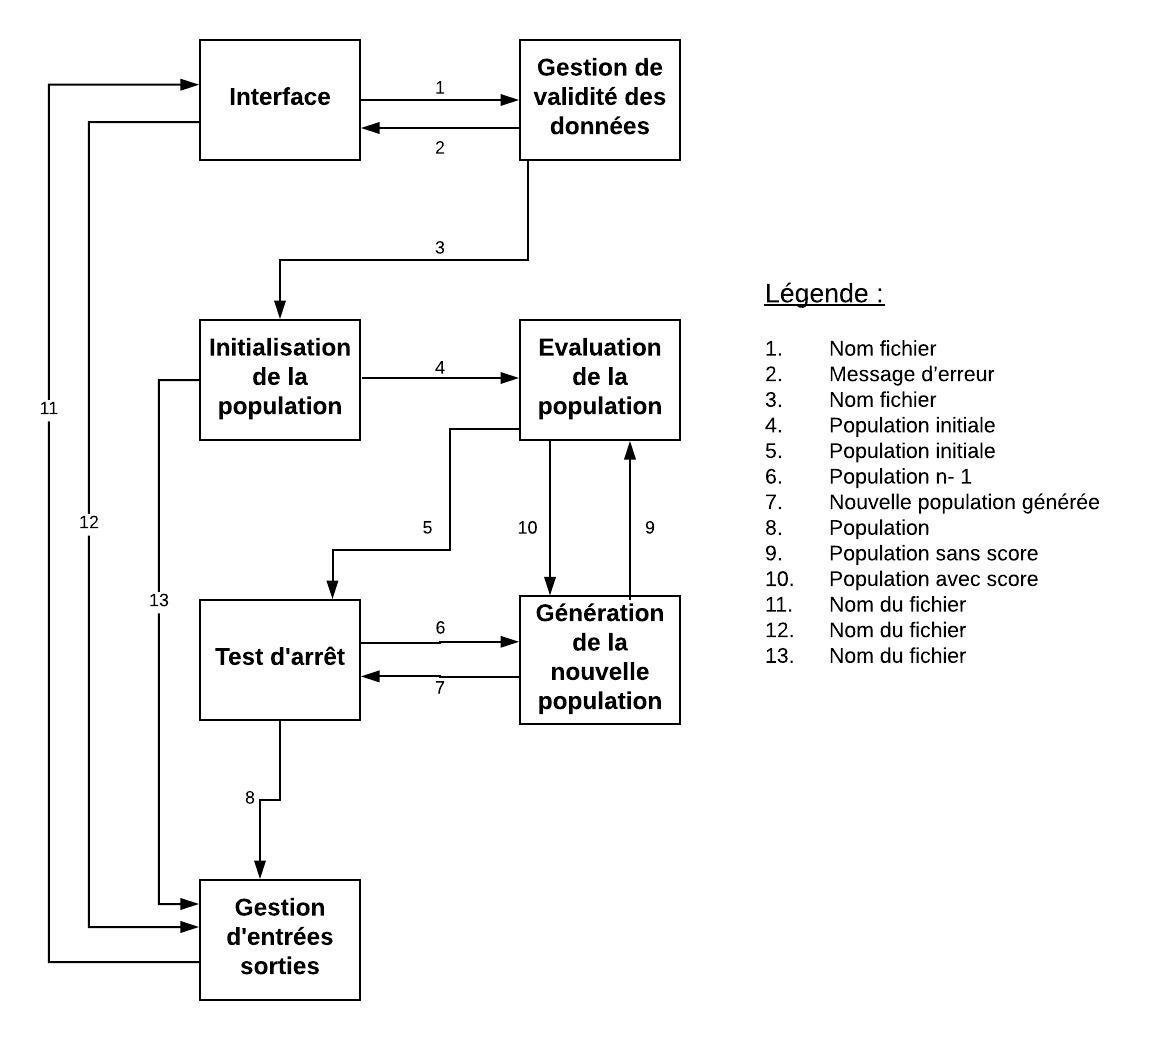
\includegraphics{OrganigrammeV5.jpeg}}
\end{document}
